% Publication vector schematic; no numerical solution is represented.
% Lettering: width 2A, height B, hole center (x_c,y_c), hole radius R.
% Global origin at the midpoint of the left edge, consistent with Stage I.
\begin{figure}[htbp]
  \centering
  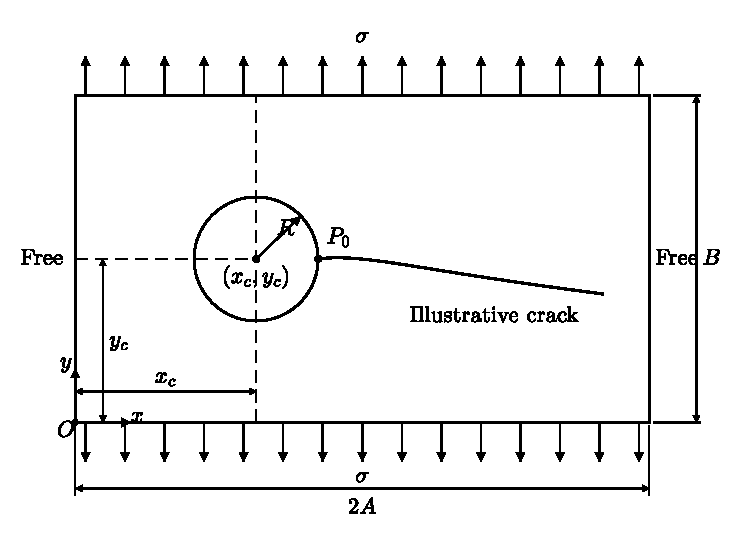
\includegraphics[width=0.94\linewidth]{figures/geometry_loading/specimen_geometry.pdf}
  \caption{Geometry and tensile loading of the plate with an eccentric
  circular hole. The plate has width $2A$ and height $B$, and the hole
  center and radius are $(x_c,y_c)$ and $R$. The coordinate origin is at
  the midpoint of the left edge; the vertical edges, hole boundary, and
  crack faces are traction free. Arrows show the direction of the applied
  tractions, both labeled by the unsigned magnitude $\sigma$.
  The smooth curvilinear crack is schematic, not a prescribed or solved path.}
  \label{fig:geometry-loading}
\end{figure}
